\documentclass[aspectratio=169]{beamer}
\usepackage{pgf}
\usepackage{multimedia}
\usepackage{colortbl,tabularx,mathrsfs,calligra,xcolor}
\usepackage{amsmath,amsfonts,amssymb,amsthm}
\usepackage{ragged2e}
\usepackage{setspace}
\usepackage{filecontents}
\usepackage{caption}
\usepackage{subcaption}
\usepackage{contour}
\usepackage{animate}
\usepackage{fancybox}
\usepackage{wrapfig}
\usepackage{multirow}
\usepackage{multicol}
\usepackage{pgfplots, tkz-euclide,calc}
    \usetikzlibrary{patterns,snakes,shapes.arrows,shapes.geometric,arrows}
\usepackage{listings}
\usepackage{enumitem}
\usepackage{pifont}
\usepackage[scaled]{berasans}
    \renewcommand*\familydefault{\sfdefault}  %% Only if the base font of the document is to be sans serif
\usepackage[T1]{fontenc}
\usepackage{hyperref}
\hypersetup{
    filecolor=magenta,      
    urlcolor=cyan,
    pdftitle={Overleaf Example},
    pdfpagemode=FullScreen,
    }
\renewcommand*\familydefault{\sfdefault} %% Only if the base font of the document is to be sans serif

\graphicspath{{C:/Users/teoso/OneDrive/Documents/Asisten Dosen & Lab/Asisten Laboratorium/Alpro 1/PPT/Graphicx/}}

\definecolor{HIMAmuda}{HTML}{01D1FD}
\definecolor{HIMAtua}{HTML}{02016A}
\definecolor{HIMAabu}{HTML}{CBCBCC}
\definecolor{PastelGreen}{HTML}{77DD77}
\definecolor{pgray}{rgb}{0.5,0.5,0.5}
\definecolor{pblue}{rgb}{0.13,0.13,1}
\definecolor{pgreen}{rgb}{0,0.5,0}
\definecolor{pred}{rgb}{0.9,0,0}
\definecolor{pgrey}{rgb}{0.46,0.45,0.48}
\definecolor{pcyan}{HTML}{D4EFFC}
\definecolor{lblue}{HTML}{00AEEF}
\definecolor{input}{HTML}{AAE1FA}
\definecolor{bg}{rgb}{0.95, 0.95, 0.92}
\definecolor{vscode}{HTML}{282A36}

\usetheme{Madrid}

\setbeamercolor{palette primary}{bg=HIMAtua,fg=white}
\setbeamercolor{palette secondary}{bg=HIMAmuda,fg=black}
\setbeamercolor{palette tertiary}{bg=HIMAabu,fg=black}
\setbeamercolor{palette quaternary}{bg=HIMAmuda,fg=white}
\setbeamercolor{structure}{fg=HIMAmuda} % itemize, enumerate, etc
\setbeamercolor{section in toc}{fg=HIMAtua} % TOC sections
\setbeamercolor{block title alerted}{fg=white,bg=magenta}
\setbeamercolor{block body alerted}{fg=black!90,bg=pink}

\usefonttheme{professionalfonts}
\setbeamertemplate{theorems}[numbered]
\setbeamertemplate{itemize items}[circle]

\usebackgroundtemplate{%
\tikz[overlay,remember picture] \node[opacity=0.1, at=(current page.center)]{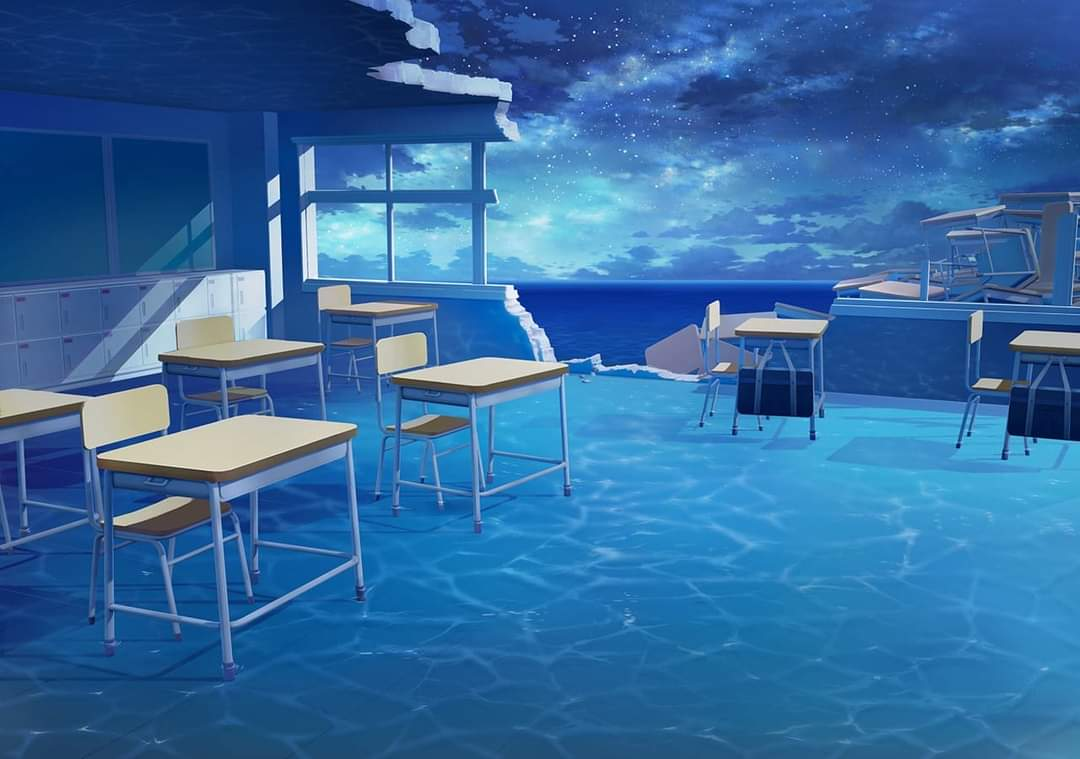
\includegraphics[width=\paperwidth]{plana class}};
}

\renewcommand\thesubfigure{\arabic{subfigure}}
\newtheorem*{funfact}{Fun Fact}
\newtheorem*{definisi}{Definisi}
\newtheorem{teorema}{Teorema}
\theoremstyle{definition}
\newtheorem{latihan}{Latihan}
\newtheorem*{contoh}{Contoh}
\newtheorem*{masalah}{Masalah}
\newcommand{\R}{\mathbb{R}}

\AtBeginEnvironment{contoh}{%
    \setbeamercolor{block title}{use=example text,fg=white,bg=example text.fg!75!black}
    \setbeamercolor{block body}{parent=normal text,use=block title example,bg=block title example.bg!10!bg}
}

\AtBeginEnvironment{funfact}{%
  \setbeamercolor{block title}{fg=white,bg=PastelGreen!50!HIMAmuda} % Set title background to pastel green and text to white
  \setbeamercolor{block body}{parent=normal text,bg=PastelGreen!50!HIMAmuda!30!white} % Set body background to a lighter pastel green
}
\AtBeginEnvironment{definisi}{
    \setbeamercolor{block title}{fg=white,bg=HIMAtua}
    \setbeamercolor{block body}{parent=normal text,bg=HIMAtua!30!white}
}
\AtBeginEnvironment{teorema}{
    \setbeamercolor{block title}{bg=darkgray,fg=white}
    \setbeamercolor{block body}{parent=pallette tertiary,bg=HIMAabu!30!white}
}
\AtBeginEnvironment{latihan}{%
  \setbeamercolor{block title}{fg=white,bg=PastelGreen} % Set title background to pastel green and text to white
  \setbeamercolor{block body}{parent=normal text,bg=PastelGreen!30!white} % Set body background to a lighter pastel green
}
\AtBeginEnvironment{masalah}{%
  \setbeamercolor{block title}{fg=white,bg=teal} % Set title background to pastel green and text to white
  \setbeamercolor{block body}{parent=normal text,bg=teal!30!white} % Set body background to a lighter pastel green
}

\renewcommand{\arraystretch}{1.3}
\renewcommand{\lstlistingname}{Kode}

\usepackage{listings}

\lstdefinestyle{standard}{
    language            = Java,
    showspaces          = false,
    showtabs            = false,
    breaklines          = true,
    showstringspaces    = false,
    breakatwhitespace   = true,
    commentstyle        = \color{pgray},
    keywordstyle        = \color{pblue},
    stringstyle         = \color{pgreen},
    basicstyle          = \footnotesize\ttfamily,
    frame               = shadowbox,
    backgroundcolor     = \color{brown!10!white},
    escapeinside        = {(*}{*)},
    numbers             = left, % {none, left, right}
    numberstyle         = \scriptsize\color{lightgray},
    numbersep           = -8pt,
    rulesepcolor        =\color{brown!50!black}
    }

\lstdefinestyle{output}{
    language=Java,
    backgroundcolor     =\color{vscode},
    basicstyle          =\footnotesize\ttfamily\color{white},
    frame               =shadowbox,
    escapeinside        ={(*}{*)},
    showspaces          =false,
    showtabs            =false,
    breaklines          =true,
    showstringspaces    =false,
    breakatwhitespace   =true,
    rulesepcolor        =\color{HIMAtua!50!white},
    rulecolor           =\color{HIMAtua!50!white},
    numbers             =none,
    }

\lstset{style=standard}

\tikzstyle{startstop} = [rectangle, rounded corners, 
minimum width=2cm, 
minimum height=1cm,
text centered, 
draw=black, 
fill=pink]

\tikzstyle{io} = [trapezium, 
trapezium stretches=true, % A later addition
trapezium left angle=70, 
trapezium right angle=110, 
minimum width=2cm, 
minimum height=1cm, text centered, 
draw=black, fill=HIMAmuda]

\tikzstyle{process} = [rectangle, 
minimum width=2cm, 
minimum height=1cm, 
text centered, 
text width=2cm, 
draw=black, 
fill=HIMAabu]

\tikzstyle{decision} = [diamond, 
minimum width=2cm, 
minimum height=1cm, 
text centered, 
draw=black, 
fill=PastelGreen]
\tikzstyle{arrow} = [thick,->,>=stealth]

\newcommand{\enter}{\raisebox{-1.8pt}{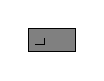
\begin{tikzpicture}[scale=0.3]
    \draw[thin,fill=gray] (0,0) rectangle (2,1);
    \draw (0.3,0.3) -- (0.7,0.3)--(0.7,0.6);     
\end{tikzpicture}}}

\newcommand{\inputscan}[1]{\raisebox{0pt}[1pt]{\colorbox{darkgray}{#1}}}

\newcommand{\inlineitem}{%
\leavevmode\usebeamertemplate{itemize item}
}

\author[Tew \& Haf]{Hafidz Mulia\\Teosofi Hidayah Agung}
\date{4 November 2024}
\title[Alpro 1 - Week 8]{Array}
\institute[Matematika ITS]{Departemen Matematika\\ Institut Teknologi Sepuluh Nopember}
\titlegraphic{{
\includegraphics[scale=0.02]{M.png}$\quad$
\includegraphics[scale=0.2]{Provicom.png}}}

\begin{document}
    {\usebackgroundtemplate{
        \tikz[overlay,remember picture] \node[opacity=0.2, at=(current page.center)]{
\includegraphics[width=\paperwidth]{bg_2}};}
    \begin{frame}
        \titlepage
    \end{frame}
    }

    \AtBeginSection{
    {\usebackgroundtemplate{
     \tikz[overlay,remember picture] \node[opacity=0.1, at=(current page.center)]{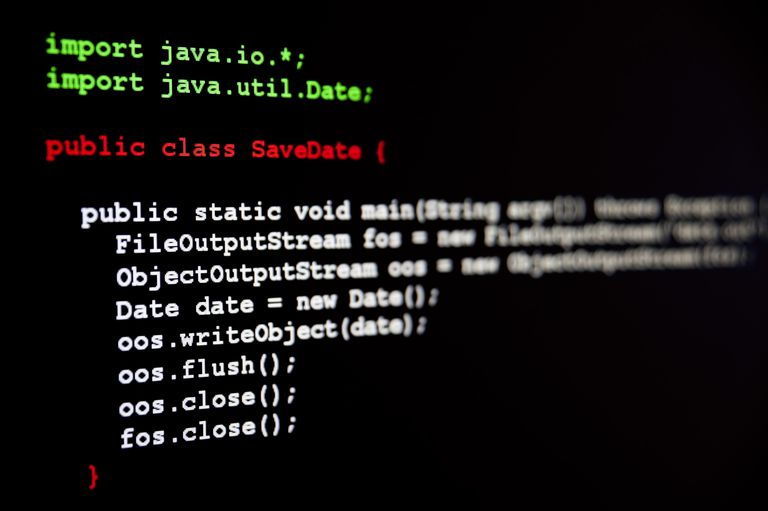
\includegraphics[width=\paperwidth]{Java code}};}
    \begin{frame}{Daftar isi}
        \tableofcontents[currentsection]
        \begin{tikzpicture}[overlay, remember picture] 
            \node at ([yshift=.5cm]current page.south east) [
                anchor = south east, 
                ] {
            \animategraphics[autoplay,loop,width=0.2\textwidth]{30}{Arisu Dance/Arisu Dance-}{0}{186}
            };
        \end{tikzpicture}
    \end{frame}}
    }
    
    \begin{frame}
        \begin{masalah}
            Di dunia ini banyak sekali objek yang memiliki \textbf{kesamaan}. Hal itu membuatnya bisa saling dikelompokkan menjadi satu kesatuan dan biasanya diberi \textbf{nama} sebagai identitas kelompok. Daripada kita menamai setiap objek tersebut satu per satu, alangkah baiknya kita buat sebuah \textbf{wadah} untuk menampung objek-objek tersebut. 
        \end{masalah}
    \end{frame}

    \section{Apa itu Array?}
    \begin{frame}
        \frametitle{\insertsection}
        \begin{definisi}
            \textbf{Array} adalah kumpulan/himpunan dari objek-objek yang memiliki kesamaan \textbf{tipe data} dan dikelompokkan dalam satu variabel. Setiap objek dalam array memiliki \textbf{indeks} yang berbeda-beda. Indeks ini digunakan untuk mengakses objek dalam array.
        \end{definisi}
    \end{frame}

    \subsection{Deklarasi Array}
    \begin{frame}[fragile]
        \frametitle{\insertsection}
        \framesubtitle{\insertsubsection}
        \begin{block}{Deklarasi Array}
            Array bisa dideklarasikan dengan cara berikut: 
        \end{block}
        \begin{lstlisting}[caption={Inisialisasi variabel array}]
    tipe_data[] nama_array; //or
    tipe_data nama_array[];
    // Contoh:
    int[] angka; //or
    int angka[];
        \end{lstlisting}
        \begin{lstlisting}[caption={Inisialisasi ukuran array}]
    tipe_data[] nama_array = new tipe_data[ukuran_array];
    // Contoh:
    int[] angka = new int[5];
        \end{lstlisting}
    \end{frame}

    \begin{frame}[fragile]
        \frametitle{\insertsection}
        \framesubtitle{\insertsubsection}
        \begin{lstlisting}[caption={Inisialisasi elemen array}]
    tipe_data[] nama_array = {objek1, objek2, objek3, ...};
    // Contoh:
    int[] angka = {1, 2, 3, 4, 5};
        \end{lstlisting}
        Paling umum tanda kurung siku \texttt{[]} diletakkan setelah tipe data dan sebelum nama variabel. 
    \end{frame}

    \subsection{Indeks Array}
    \begin{frame}[fragile]
        \frametitle{\insertsection}
        \framesubtitle{\insertsubsection}
        \begin{block}{Indeks Array}
            Indeks array dimulai dari 0 hingga $n-1$, dengan $n$ menyatakan ukuran array. Namun karena terkadang kita tidak mengetahui secara eksplisit ukuran array yang akan kita eksekusi, maka kita bisa menggunakan \textit{method} \texttt{.length} untuk mengetahui ukuran array.
        \end{block}
        \begin{lstlisting}[caption={Memberi input pada array}]
    Scanner input = new Scanner(System.in);
    int[] angka = new int[5];
    for (int i = 0; i < angka.length; i++) {
        angka[i] = input.nextInt();
    }
        \end{lstlisting}
    \end{frame}

    \begin{frame}[fragile]
        \frametitle{\insertsection}
        \framesubtitle{\insertsubsection}
        \begin{alertblock}{Out of Bound}
            Jika kita mencoba mengakses indeks array yang tidak ada, maka akan terjadi \textbf{\color{red}ArrayIndexOutOfBoundsException}. Hal ini biasanya terjadi saat kita mengeksekusi array dengan perulangan.
        \end{alertblock}
        \begin{lstlisting}[caption={Contoh eror dalam array}]
    String[] nama = {"Agas", "Agus", "Age"};
    nama[3] = "Agis"; //ArrayIndexOutOfBoundsException
        \end{lstlisting}
    \end{frame}

    \section{Display Array}
    \begin{frame}
        \frametitle{\insertsection}
        \begin{block}{Menampilkan Array}
            Misalkan kita memiliki array dengan nama \texttt{angka} yang berisi \texttt{[1, 2, 3, 4, 5]}. Kemudian kita lakukan \texttt{System.out.println(angka)}, kira-kira apa output programnya?
        \end{block}
        \onslide<2>{\begin{alertblock}{Ingat}
            Pada materi yang membahas tentang variabel, Array bertipe data \texttt{reference}. Jadi, ketika kita mencetak array, yang dicetak adalah alamat memori dari array tersebut bukan isinya.
        \end{alertblock}
        Lalu bagaimana cara menampilkan isi array?
        }
    \end{frame}

    \subsection{For-loop}
    \begin{frame}[fragile]
        \frametitle{\insertsection}
        \framesubtitle{\insertsubsection}
        \begin{block}{For-loop}
            Cara paling umum untuk menampilkan isi array adalah dengan menggunakan \texttt{for-loop}. Karena setiap elemen array memiliki indeks, maka kita bisa menggunakan indeks tersebut untuk mengakses elemen array.
        \end{block}
        \begin{lstlisting}[caption={Menampilkan array dengan for-loop}]
    int[] angka = {1, 1, 2, 3, 5};
    for (int i = 0; i < angka.length; i++) {
        System.out.print(angka[i] + " ");
    }
        \end{lstlisting}
        \begin{lstlisting}[style=output]
    1 1 2 3 5
        \end{lstlisting}
    \end{frame}

    \subsection{For-each}
    \begin{frame}[fragile]
        \frametitle{\insertsection}
        \framesubtitle{\insertsubsection}
        \begin{block}{For-each}
            Selain menggunakan \texttt{for-loop}, kita juga bisa menggunakan \texttt{for-each} untuk menampilkan isi array. For-each biasanya digunakan untuk mengakses elemen array tanpa harus mengetahui indeksnya.
        \end{block}
        \begin{lstlisting}[caption={Menampilkan array dengan for-each}]
    double[] numbers = {3.5, 1.1, 2.2, 11.8, 8.9};
    for (int num : numbers) {
        System.out.print(num + " ");
    }
        \end{lstlisting}
        \begin{lstlisting}[style=output]
    3.5 1.1 2.2 11.8 8.9
        \end{lstlisting}
    \end{frame}

    \subsection{Import Arrays}
    \begin{frame}[fragile]
        \frametitle{\insertsection}
        \framesubtitle{\insertsubsection}
        \begin{block}{Import Arrays}
            Hal yang paling mudah untuk menampilkan isi array adalah dengan menggunakan \texttt{Arrays.toString()}. Sebelum menggunakan method ini, kita harus meng-import \texttt{java.util.Arrays}.
        \end{block}
        \begin{lstlisting}[caption={Arrays.toString()}]
    import java.util.Arrays;
    public class DisplayArray {
        public static void main(String[] args) {
            int[] angka = {1, 2, 3, 4, 5};
            System.out.println(Arrays.toString(angka));
        }
    }
        \end{lstlisting}
        \begin{lstlisting}[style=output]
    [1, 2, 3, 4, 5]
        \end{lstlisting}
    \end{frame}

    \section{Array Multidimensi}
    \begin{frame}[fragile]
        \frametitle{\insertsection}
        \begin{definisi}
            \textbf{Array multidimensi} adalah array yang memiliki lebih dari satu dimensi. Array ini biasanya digunakan untuk menyimpan data yang memiliki struktur tertentu, seperti matriks, tabel, dan lain-lain.
        \end{definisi}
        \begin{lstlisting}[caption={Deklarasi array 2D}]
    tipe_data[][] nama_array = new tipe_data[baris][kolom];
    // Contoh:
    int[][] matriks = new int[2][3];
        \end{lstlisting}
    \end{frame}

    \begin{frame}
        \frametitle{\insertsection}
        \begin{block}{Array 2D}
            Array 2D biasanya digunakan untuk menyimpan data yang memiliki struktur matriks. Array ini memiliki dua indeks, yaitu indeks baris dan indeks kolom.
        \end{block}
        \begin{contoh}
            Misalkan kita memiliki matriks \[A = \begin{bmatrix} 1 & 2 & 3 \\ 4 & 5 & 6 \end{bmatrix}\] kita bisa merepresentasikan matriks tersebut dengan array 2D sebagai berikut:
        \end{contoh}
    \end{frame}

    \begin{frame}[fragile]
        \frametitle{\insertsection}
        \begin{lstlisting}[caption={Matriks dengan Array 2D}]
    int[][] matriks = {{1, 2, 3}, {4, 5, 6}};
    for (int i = 0; i < matriks.length; i++) {
        for (int j = 0; j < matriks[i].length; j++) {
            System.out.print(matriks[i][j] + " ");
        }
        System.out.println();
    }
        \end{lstlisting}
        \begin{lstlisting}[style=output]
    1 2 3
    4 5 6
        \end{lstlisting}
    \end{frame}

    \begin{frame}
        \frametitle{\insertsection}
        \begin{alertblock}{Catatan}
            Pada dasarnya array multidimensi adalah array yang berisi array. Sehingga jika kita hanya mengakses array \textit{luar}, maka yang dicetak adalah alamat memori dari array \textit{dalam}.
        \end{alertblock}
    \end{frame}

    \section{Latihan}
    \begin{frame}
        \begin{latihan}
            Buatlah program yang menghitung jumlah elemen dalam array\\
            Contoh: \texttt{\{9, 8, 6, 14, 0\}} $\to$ \texttt{37}
        \end{latihan}
        \begin{latihan}
            Buatlah program yang mencari nilai maksimum dalam array\\
            Contoh: \texttt{\{66, 78, 90, 16, 7\}} $\to$ \texttt{90}
        \end{latihan}
        \begin{latihan}
            Buatlah program yang menjumlahkan dua buah matriks yang dimana ukuran matriks tersebut harus sama
        \end{latihan}
    \end{frame}
\end{document}